% 文档类型
\documentclass{article}

% 引入宏包
\usepackage{graphicx}
\usepackage{amsmath,amsfonts}
\usepackage{algorithm, algorithmic}
\usepackage{hyperref}

% 标题、作者等信息
\title{\LaTeX \, Example}
\author{Zhang San}
\date{2019.07}

% 自定义命令
\newcommand{\Prob}{\mathbb{P}}

% 正文
\begin{document}

\maketitle

\begin{abstract}
This is the abstract. This is the abstract. This is the abstract. This is the abstract. This is the abstract. This is the abstract. This is the abstract. This is the abstract.This is the abstract. This is the abstract. This is the abstract.This is the abstract.This is the abstract.This is the abstract.
\end{abstract}


% 节
\section{Introduction} 

% 小节
\subsection{Background}

This is a \LaTeX document.


\subsection{Math}

This is an stochastic differential eqation: 
\begin{equation}\label{sde}
\left\{
\begin{aligned}
	dX(t) &= f\big(X(t)\big)dt + \sum_{r=1}^m g_r\big(X(t)\big) \circ dW_r(t), \quad t\in [0, T],\\
	X(0) &= X_0,
\end{aligned}\right.
\end{equation}
where $f(x) \in \mathbb{R}^n$ is called the drift.

Equation \ref{sde} is an SDE.


\begin{itemize}
	\item First .....
	\begin{itemize}
		\item aaaaa
		\item bbbbb
	\end{itemize}
	\item Second .....
	\item Third ....
\end{itemize}

\begin{enumerate}
	\item First .....
	\item Second .....
	\begin{itemize}
		\item aaaaaaaa
		\item bbbbbbbb
	\end{itemize}
	\item Third ....
\end{enumerate}

\subsection{Figure}

Figure \ref{fig1} is a path of an one dimensional Wiener Process.

\begin{figure}[htbp]
	\centering
	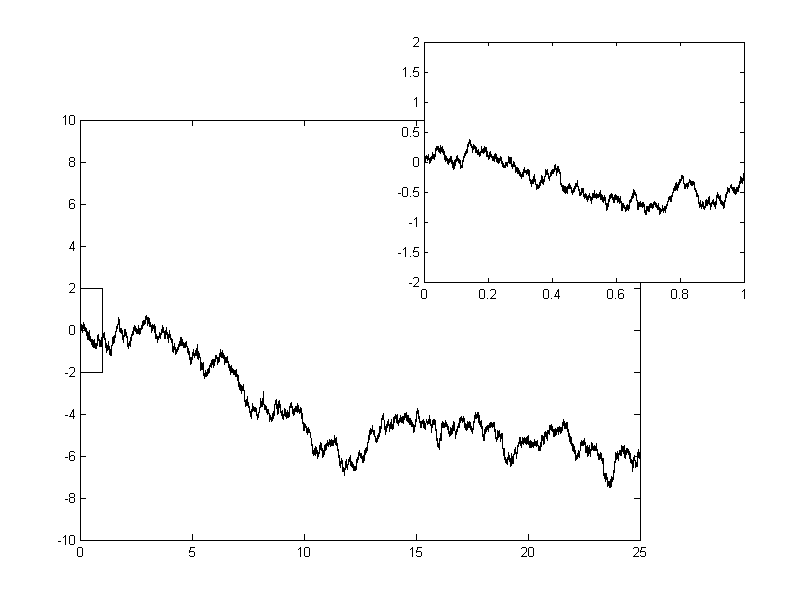
\includegraphics[width=0.7\linewidth]{Wiener_process_zoom}
	\caption{This is the figure caption.}
	\label{fig1}
\end{figure}

\subsubsection{Table}

\begin{table}[htbp]
	\centering
	\begin{tabular}{l|lllll}
		\hline
		A & B & C & D & E  & F \\ \hline
		1 & 2 & 3 & 4 & 5  & 6 \\
		7 & 8 & 9 & 10 & 11 & 12 \\ \hline
	\end{tabular}
	\caption{This is the table caption.}
\end{table}



\subsection{Citation}

This is a citation\cite{Silver2016Mastering,Mnih2015Human,pmlr-v48-mniha16}.


\subsection{Algorithm}

\begin{algorithm}
	\caption{Calculate $y = x^n$}
	\label{alg1}
	\begin{algorithmic}
		\REQUIRE $n \geq 0 \vee x \neq 0$
		\ENSURE $y = x^n$
		\STATE $y \leftarrow 1$
		\IF{$n < 0$}
		\STATE $X \leftarrow 1 / x$
		\STATE $N \leftarrow -n$
		\ELSE
		\STATE $X \leftarrow x$
		\STATE $N \leftarrow n$
		\ENDIF
		\WHILE{$N \neq 0$}
		\IF{$N$ is even}
		\STATE $X \leftarrow X \times X$
		\STATE $N \leftarrow N / 2$
		\ELSE[$N$ is odd]
		\STATE $y \leftarrow y \times X$
		\STATE $N \leftarrow N - 1$
		\ENDIF
		\ENDWHILE
	\end{algorithmic}
\end{algorithm}



% 参考文献样式,根据需要选择
\bibliographystyle{IEEEtran}

% 参考文献文件
\bibliography{references.bib}

\end{document}
